\chapter{Introduction} \label{chap:intro}
This chapter explains the problems faced by the companies during Software development (see section \ref{intro:section:problems}), our Research approach (see section \ref{intro:section:research}), and finally, our solution approach (see section \ref{intro:section:solution}).

\section{Motivation}
Over the last decade, Software development had a tremendous impact with increasing customer demand and requirements \cite{article:swdemand:ahmed}. 
The product designers responsible for designing various product variants are unsure which variant would be most liked by the customers.
Similarly, increasing product complexity and ambiguity significantly impact software development. 
So, the developers have come up with different techniques to meet this requirement criteria.
Early user feedback from potential customers in the industry is crucial for creating successful software products because of the growing market uncertainties, and consumers' desire to receive integrated solutions to their issues rather than unique software developments \cite{misc:businessmodels:teece}.
With the increasing complexity of products, it becomes challenging to determine user requirements making it more difficult for developers to assess their opinions.
As a result, the developers of these products are biased toward some requirements and can ignore what the user wants. 
We must detect the user's needs and requirements to reduce these risks early. 
Giving users a ``partially functioning'' system is the most excellent method to determine their requirements and suggestions \cite{journal:prototyping:davis}.
This ensures that the developers with high uncertainties in the early product development can validate by testing the underlying assumptions \cite{misc:lean:steve}.
Developers can use this feedback to validate the most critical assumptions about the software product. 
This validation can decide whether to add, remove or update a feature \cite{article:experiments:lindgren}. 
This process of determining the best fit for the product through user feedback is called experimentation.
There has been an increase in interest in the types of experimentation that can take place in product development. 
Software products have shown the benefits of conducting experiments in many use cases with incremental product improvement \cite{article:controlled:experiements}.
In experimentation, the product designers design different UI variants (e.g., buttons with different colors), and the developer integrates these variants and assigns them to a distinct group of users. 
As per some evaluation criteria (e.g., more clicks on the button), the variant with better results is deployed for the entire set of users.
So, an experiment can be valuable when it improves the software products.
Hence, for experiments to be successful, they should offer one or more solutions that will benefit users.

\section{Problem Statement}
\label{intro:section:problems}
This section explains the current problems faced by developers during software development. 
We define three problems and determine the research and the solution approach for the same.

\paragraph{Problem 1:} Product designers create many UI prototypes, and the developers implement them.
To determine the best variant, the developers create experiments with the users. 
This concrete implementation of designs uses a lot of resources and time for the developers.
Therefore, the product designers need to be integrated into the development process so that they would be able to create experiments independent of the developers.

% \paragraph{Problem 2:} (Use design principles)

\paragraph{Problem 2:} When the product designers develop the prototypes, testing them with many users is difficult as the product is still not developed.
Therefore, it is not easy to conclude a ``winner'' variant with a small amount of data as it is statistically difficult to prove one of the variants outperforms the others \cite{article:usability:smalldata}.
Therefore, it is necessary to develop an idea that the designers can use to determine the best prototype or variant with a small group of users.

\paragraph{Problem 3:} Most often, the software application collects data from the experiments. 
Some data is used in Qualitative analysis, while others are in Quantitative analysis.
Many companies fail to reap the benefits of using both Qualitative and Quantitative analysis.
Similarly, not all the data is used in the analysis phase reducing the software applications to improve based on customer feedback \cite{article:datadrive:brian}.
Therefore, finding a solution that combines qualitative and quantitative data analysis is necessary.

\section{Research Approach}
\label{intro:section:research}
\begin{figure}[ht]
    \centering
    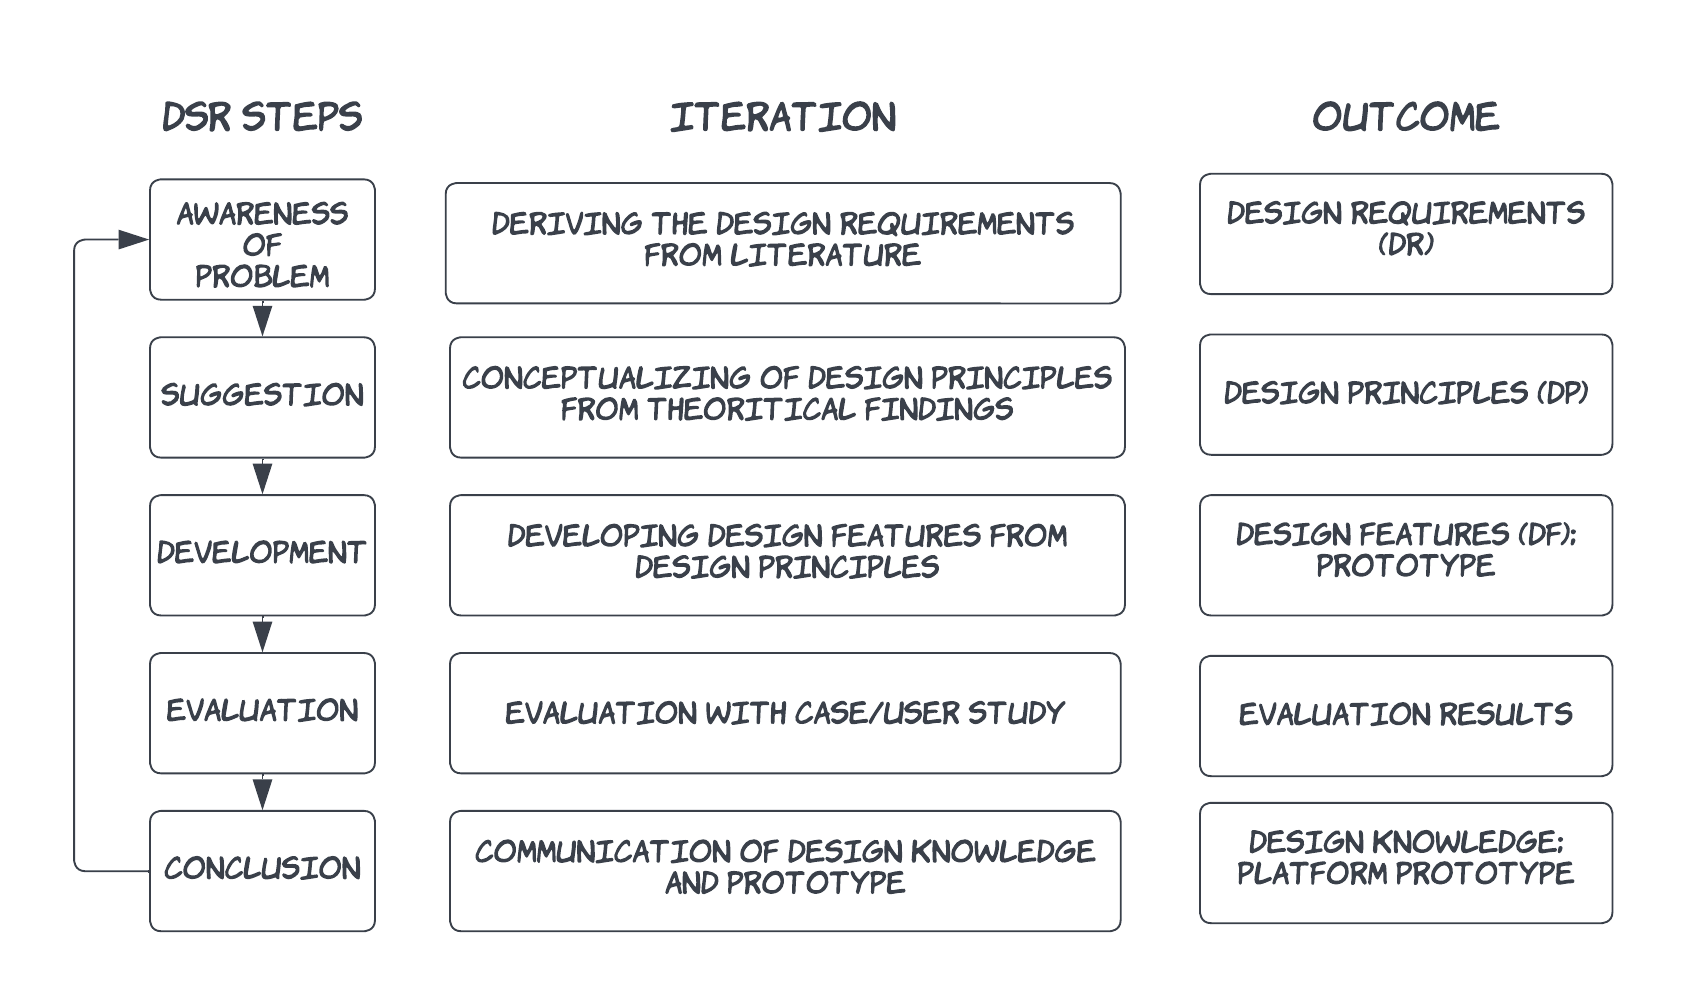
\includegraphics[scale=0.2]{images/solution-ideas/DSRcycle.png}
    \caption{Design Science Research Cycle \cite{paper:designprinciple:vk}}
    \label{intro:fig:dps}
\end{figure}
The process of creating experiments and testing their variants is usually not systematically arranged, creating anomalies, and leading to unsuccessful experiments.
Therefore, this section identifies the Research Question (RQ) and defines an approach to answer the question.

\paragraph{RQ:}How to develop a platform suitable for product designers to conduct experiments on UI prototypes, increasing its usability and, at the same time, independent of developers?

% The process of creating experiments and testing their variants is usually not systematically arranged, creating anomalies, and leading to unsuccessful experiments.
To answer this question, we will conduct a design science research (DSR) study where the software designers iteratively validate their prototypes with the users to obtain some Design Principles (DPs) defined for the whole process of experimentation \cite{paper:designprinciple:vk}. 
Here, DPs capture and codify that knowledge by focussing on the implementer, the aim, the user, the context, the mechanism, the enactors, and the rationale \cite{paper:designprinciple:gregor}. 
The DPs explain the design information that develops features for software applications.
We propose to use the variation of the cycle of Kuechler and Vaishnavi \cite{paper:designprinciple:vk} consisting of five iteratively conducted steps (see figure \ref{intro:fig:dps}). 
First, we identify the 
\texttt{(1) Awareness of the Problem} and provide a
\texttt{(2) Suggestion of a possible solution}. Next, we work on the 
\texttt{(3) Development of the software artifact} and conduct an 
\texttt{(4) Evaluation} of it. Based on the evaluation results, we provide 
\texttt{(5) Conclusions} \cite{misc:crowdsourcing:sg}.
From each step of the DSR, we have an iteration cycle and an outcome (e.g., Awareness of the Problem leads to finding Design Requirements, Design Principles (DPs) can be found from the Suggestion of the solution, Development of the software artifact leads to finding the Design Features and the Prototype, etc.) as shown in figure \ref{intro:fig:dps}.
Therefore through the use of DSR, a group of issues is resolved by concentrating on a single issue and abstracting the consequences of the resolution.


\section{Solution Approach}
\label{intro:section:solution}
To solve the problems mentioned above, the designers should be able to create UI prototypes and experiments on their own on a set of users.
Since we do not have a large set of users for testing the prototypes, we use supervised task-based usability testing \cite{article:dataanalysis:supervisedtest}.
The fundamental principle of task-based usability testing is to have the users attempt to use the prototypes to do certain activities or tasks (e.g., Locate a movie M1) and get feedback (e.g., the time required for the task to be completed by the user).
We propose to use \texttt{Low-code} or \texttt{No-Code} approach to achieve this.
This approach helps to have a UI interface for the designers to understand, develop, and create experiments and tasks with the software prototypes \cite{paper:lowcode:khorram}.
So, the designers would be able to test the UI prototypes, assign them to the users, get feedback from the users and decide on the best prototype.
At the same time, the Low-code has become more accessible for Model-driven development.
Therefore, we plan to create models for the UI prototypes and have the feasibility for creating experiments and tasks. 
Because of using the models, it is easier to store the prototypes in the database and conduct experiments with the users. 

\begin{figure}[ht]
    \centering
    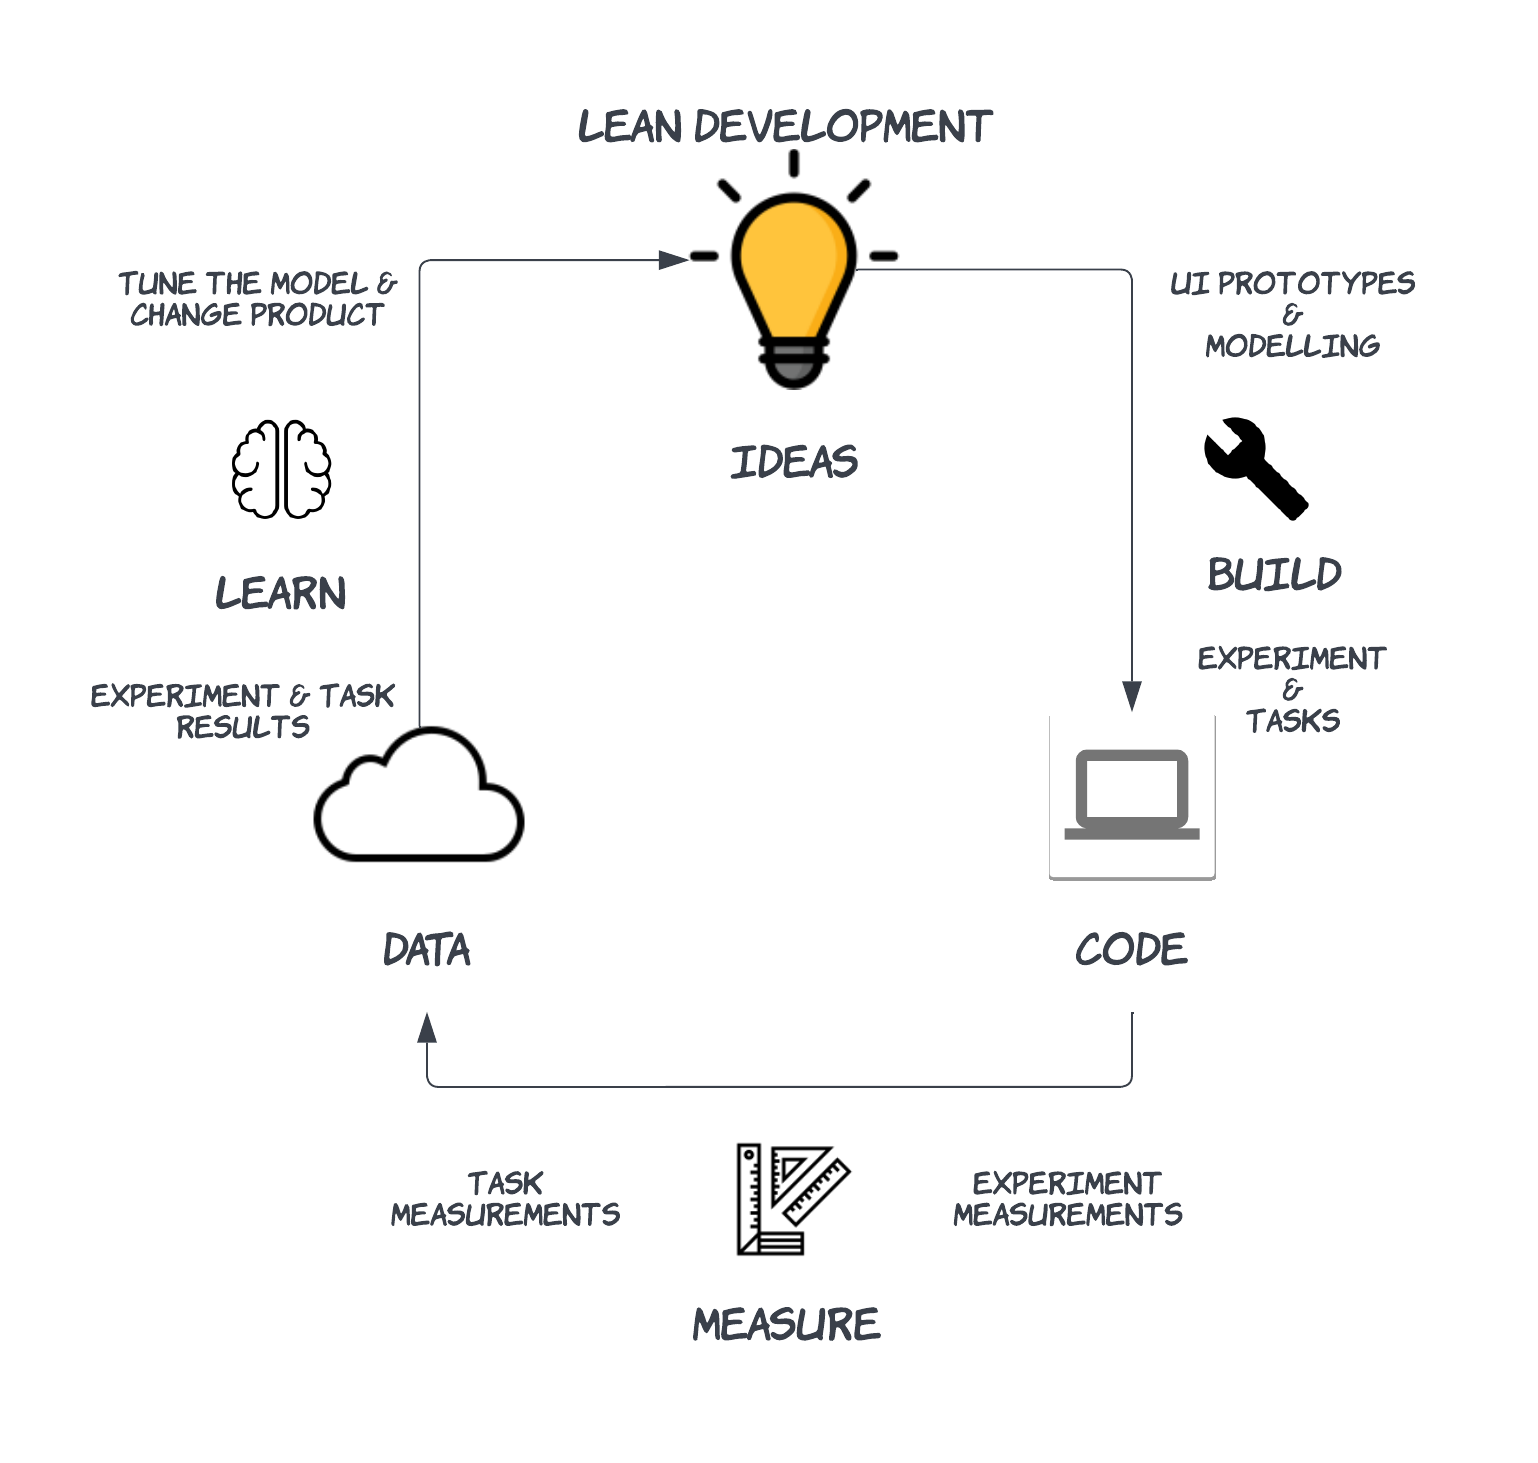
\includegraphics[scale=0.15]{images/solution-ideas/LEAN.png}
    \caption{LEAN Development technique}
    \label{intro:fig:lean}
\end{figure}

In our solution, we use the LEAN development technique (see figure \ref{intro:fig:lean}) for development as it is used to develop customers friendly products \cite{article:lean:hart}.
Using LEAN, the company creates a Minimum Viable Product (MVP) throughout development, tests it with potential customers, and leverages their input to make incremental changes.
While this technique can be used for every product, there are also approaches specific to software products.
LEAN development technique can be divided into a Build, Measure, and Learn cycle. 
In the \texttt{(1) Build} phase, we plan to create the \texttt{UI Prototypes}, \texttt{Models}, \texttt{Experiments}, and \texttt{Tasks} for the users.
In the \texttt{(2) Measure} phase, we plan to assign the Experiments and Tasks to the users and measure the \texttt{Task and the Experiment measurements} and perform some analysis on the data received. 
And finally, in the \texttt{(3) Learn} phase, we display the \texttt{Analyses results}, \texttt{Tune} our models to decide the better variant among the others, and \texttt{Modify} the prototype.
As per the figure \ref{intro:fig:lean}, we complete one cycle of iteration and start a new one with the updated prototype.
The solution approach is explained more in detail in Chapter \ref{chap:solutionideas}.

% To solve the first problem, the developers focus more on automating the software code rather than coding everything stated in the product requirements \cite{article:prototyping:hoffnagle}.
% This approach is formally known as a \texttt{Low-code} or \texttt{No-Code} approach.
% So, this approach helps to have a UI interface for the non-developers to understand and develop the software products \cite{paper:lowcode:khorram}.
% One approach to support the product owners in developing the variants is UI Prototyping. 
% UI prototyping creates new UI variants using predefined UI elements (e.g., Drag and drop the UI element Button into the screen).
% This helps product owners to be creative and innovative because it gives them visual feedback.
% So, if UI prototypes are developed in a low-code technique, they would be lightweight software that helps the product owner develop various prototypes and conduct experiments on the users.
% According to Cabot et al. \cite{paper:lowcode:cabot}, the low-code has become more accessible for Model-driven development. 
% Similarly, while creating prototyping, the software should have connections between the screens (e.g., clicking on a button should go to the next screen), and this logic can be achieved using Models.
% Models are used broadly in prototyping because a model represents or describes the aspects of the systems that cannot be described adequately in a system of interest \cite{paper:prototyping:luqi}.
% Moderately accurate models can be created using an iterative approach in software development by getting continuous feedback from the users.


% To solve the \texttt{second} problem, we use supervised task-based usability testing \cite{article:dataanalysis:supervisedtest}.
% The fundamental principle of usability testing is to have real users attempt to use the software application to do certain activities.
% Observing users interact with an interface is the most efficient way to determine what functions well and what doesn't.
% The users will undertake realistic actions, giving us qualitative insights into the problems that users are experiencing and enhancing the design with these insights \cite{misc:usability:tasks}.
% These activities can be the tasks or scenarios (e.g., Locate a movie M1) for the users to complete and analyze (e.g., the time/clicks required to locate the Movie M1).

% To solve the \texttt{third} problem, the models should use data to measure the experiments' success for improvement. This process is called a Data-driven development approach. 
% This approach uses meaningful, actionable consumer feedback regarding the effects of the product experiments by using the \texttt{Qualitative and Quantitative} data analysis.
% Using a combination of qualitative and quantitative data can improve an evaluation by ensuring that the strengths of another balance the limitations of one type of data confirming that the knowledge is enhanced by integrating different techniques.




% In our solution, we use the LEAN development technique (see figure \ref{intro:fig:lean}) for development as it is used to develop customers friendly products \cite{article:lean:hart}.
% Using LEAN, the company creates a Minimum Viable Product (MVP) throughout development, tests it with potential customers, and leverages their input to make incremental changes.
% While this technique can be used for every product, there are also approaches specific to software products.
% LEAN development technique can be divided into a Build, Measure, and Learn cycle. 
% In the \texttt{(1) Build} phase, we plan to create the \texttt{UI Prototypes}, \texttt{Models}, \texttt{Experiments}, and \texttt{Tasks} for the users.
% In the \texttt{(2) Measure} phase, we plan to assign the Experiments and Tasks to the users and measure the \texttt{Task and the Experiment measurements} and perform some analysis on the data received. 
% And finally, in the \texttt{(3) Learn} phase, we display the \texttt{Analyses results}, \texttt{Tune} our models to decide the better variant among the others, and \texttt{Modify} the prototype.
% As per the figure \ref{intro:fig:lean}, we complete one cycle and start a new iteration.
% The solution approach is explained more in detail in Chapter \ref{chap:solutionideas}.